\documentclass[border=4mm]{article}
\usepackage{tikz}
\usetikzlibrary{arrows.meta,positioning}
\title{Max-Min Flow}
\begin{document}
    \maketitle
    \tableofcontents
    \section{Overview Of Flow Network}
    \begin{enumerate}
        \item Introduction to Flow Graph, Maximum Flow and other terminologies.
        \item Ford- Fulkerson Algorithm for computation of maximum flow and its limitations.
        \item Edmond-Karp Algorithm \& its implementation
        \item Solving a related problem.
    \end{enumerate}

    \section{Network}
        A network is a directed graph G with vertex set V and edge set E combine with a function C which maps all edges (say e) to some non-negative integer (or real numbers) which is called the capacity of edge e.

    \section{Flow Network}
        Additionally in the network if we label $2$ nodes / vertices as \textbf{source} and \textbf{sink} this is called a flow network.
    
    \section{Flow}
        A function F which maps all edges (say e) to some non-negative integer (or real numbers) which is called the flow through edge e.
        The function has to fulfill $2$ conditions.
        \begin{enumerate}
            \item Flow of an edge can not exceed the capacity of that edge. \\
            $f(e) \leq c(e)$
            \item For all vertex $u$ (except \textbf{source} and \textbf{sink}), the sum of \textbf{\emph{in-flow}} should be equal to sum of \textbf{\emph{out-flow}}
        \end{enumerate}
    
    For source and sink, outFlow of source = inFlow of sink

    \section{Example}
    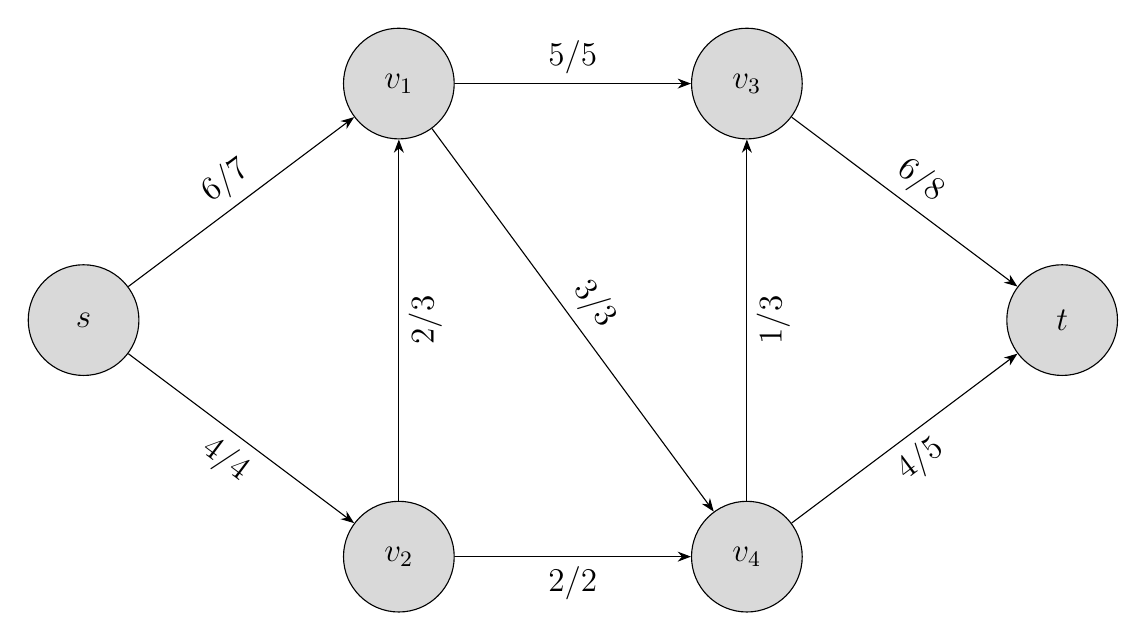
\begin{tikzpicture}[
        mycircle/.style={
        circle,
        draw=black,
        fill=gray,
        fill opacity = 0.3,
        text opacity=1,
        inner sep=2pt,
        minimum size=40pt,
        font=\large},
    myarrow/.style={-Stealth},
    node distance=2cm and 3cm
    ]
    \node[mycircle] (c1) {$s$};
    \node[mycircle,below right=of c1] (c2) {$v_2$};
    \node[mycircle,right=of c2] (c3) {$v_4$};
    \node[mycircle,above right=of c1] (c4) {$v_1$};
    \node[mycircle,right=of c4] (c5) {$v_3$};
    \node[mycircle,below right=of c5] (c6) {$t$};

    \foreach \i/\j/\txt/\p in {% start node/end node/text/position
        c1/c2/{4/4}/below,
        c1/c4/{6/7}/above,
        c2/c3/{2/2}/below,
        c3/c6/{4/5}/below,
        c4/c5/{5/5}/above,
        c5/c6/{6/8}/above,
        c3/c5/{1/3}/below,
        c2/c4/{2/3}/below,
        c4/c3/{3/3}/above}
        \draw [myarrow] (\i) -- node[sloped,font=\large,\p] {\txt} (\j);


    % draw this outside loop to get proper orientation of 10
    \end{tikzpicture}
\end{document}